\chapter{Datos}

\section{Flujo de los datos}

La presente sección describe, de pies a cabeza, el flujo que los datos atraviesan desde su origen hasta su destino final en el perfil del estudiante. En particular, se detallan las fuentes de los datos, el proceso de \gls{ETL} al que son sometidos, su representación como recursos accesibles mediante una \gls{API REST} y su posterior consumo por el frontend, correspondiente al perfil del estudiante.

\subsection{Fuentes de datos}

La información que se utiliza como fuente para el perfil del estudiante es provista por la Oficina de Registro y otras dependencias de la universidad. %TODO: Mirar quién exactamente los provee
Esa información se encuentra en archivos PARQUET y XLSX almacenados en la nube mediante Microsoft Azure Blob Storage, en diversas cuentas de almacenamiento Azure Storage Account. Para el perfil del estudiante se hace uso de diez de esos archivos, distribuidos en dos cuentas de almacenamiento. Todos los archivos utilizados, junto con su ubicación en cuentas de almacenamiento y directorios, se muestran en la figura \ref{fig:blob_storage}. 

\begin{figure}[h]
    \centering
    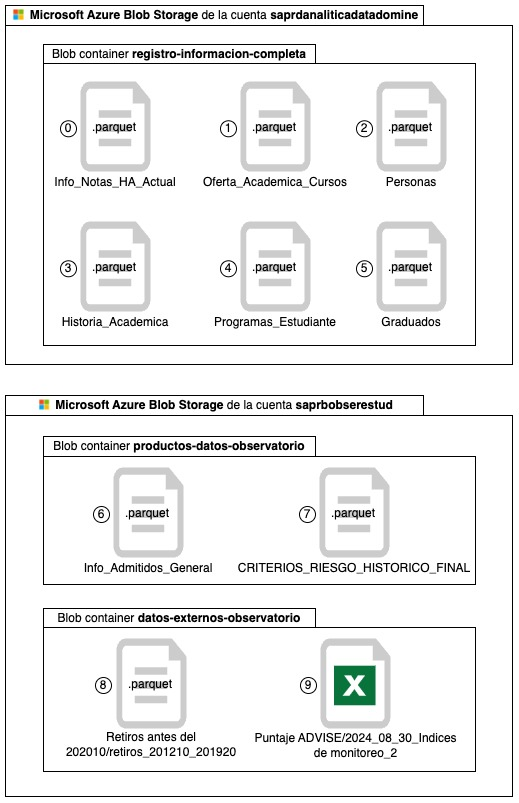
\includegraphics[width=0.7\textwidth]{img/blob_storage.jpg}
    \caption{Archivos fuente y estructura de directorios en Azure Blob Storage}
    \label{fig:blob_storage}
\end{figure}

\subsection{Procesamiento de los datos}

La recuperación y el procesamiento de los datos se realizan mediante un \textit{pipeline} de analítica implementado en cuadernos de Jupyter en Python, en colaboración con los estudiantes Santiago Martínez Novoa y Manuel Felipe Porras Tascón\footnote{Mi más sincero agradecimiento a ambos: a Manuel, en aquel momento estudiante de la Maestría en Ingeniería de la Información, por su valiosa labor al crear y trabajar inicialmente en el cuaderno; y a Santiago, entonces estudiante de Ingeniería de Sistemas y Computación, por tomar la posta, mejorar y mantener este trabajo. Sin ellos, este proyecto no habría sido posible.}.
El pipeline de analítica realiza las tres etapas clásicas de un proceso de \gls{ETL}: extracción, transformación y carga de los datos.


\subsubsection{Extracción de los datos}

El proceso de extracción consiste de tomar información determinada de cada uno de los archivos presentados en la figura \ref{fig:blob_storage}. La tabla \ref{tab:extraccion} detalla el orden en el que se realiza cada extracción, describe la información que se extrae y especifica el archivo fuente del cual se obtiene, empleando la numeración de los archivos definida en la figura \ref{fig:blob_storage}.

\begin{table}[h]
  \centering
  \caption{Extracción de datos}
  \alternatecolors
  \begin{tabular}{cp{2.3cm}p{7cm}c}
  \hline
  \textbf{Orden} & \textbf{Información} & \textbf{Descripción} & \textbf{Archivos fuente} \\
  \hline
  1 & Histórico académico & Información de las notas obtenidas por los estudiantes en cada una de las asignaturas que han cursado. & 0 \\
  2 & Oferta \newline académica & Información de las asignaturas que se ofertan en cada uno de los semestres académicos. & 1 \\
  3 & Estudiantes & Información básica de los estudiantes. & 2, 3, 6 \\
  4 & Programas académicos & Información de los programas académicos en los que se encuentran inscritos los estudiantes. & 4 \\
  5 & Información \newline adicional \newline de retiros & Información sobre los retiros de los estudiantes para periodos anteriores al 2019-20, que no se encuentra en el Histórico académico. & 8 \\
  6 & Graduados & Información de los estudiantes que se han graduado. & 5 \\
  7 & Criterios \newline de riesgo & Información de los criterios de riesgo que se utilizan para identificar a los estudiantes en riesgo académico. & 7 \\
  8 & Advise & Información de los estudiantes tomada de la plataforma Advise. & 9 \\
  \hline
  \end{tabular}
  \label{tab:extraccion}
\end{table}

\subsubsection{Transformación de los datos}

\TODO{Sentarme con Santi a describir la transformación de los datos}

\subsubsection{Carga de los datos}

Como última etapa del procesamiento de los datos, una vez han sido transformados, se cargan en dos archivos en el Blob Storage: uno correspondiente a toda la información relacionada con cada estudiante y otro contiene la información de todas las materias cursadas por cada uno de los estudiantes. La figura \ref{fig:blob_storage_post}, que extiende la figura \ref{fig:blob_storage}, muestra la estructura de directorios y archivos en el Blob Storage tras la carga del par de archivos mencionado.

\begin{figure}[h]
    \centering
    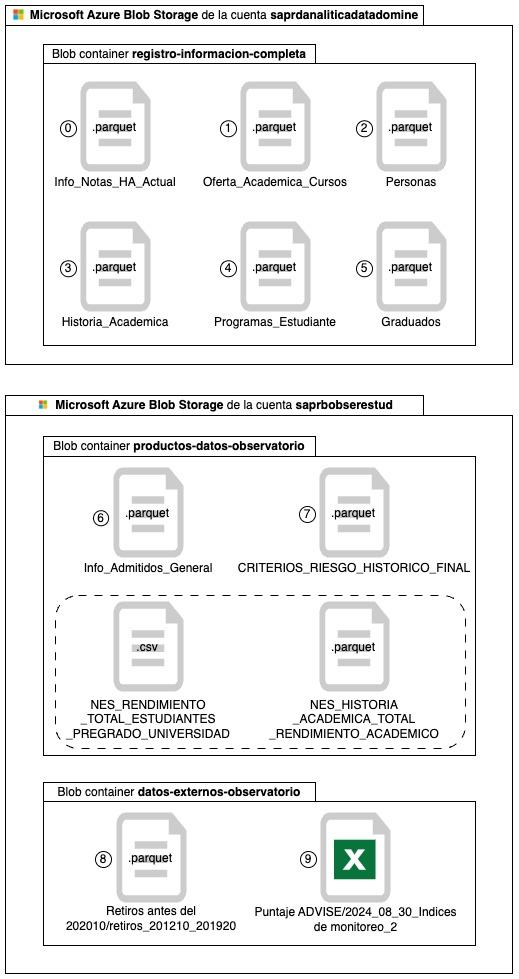
\includegraphics[width=0.7\textwidth]{img/blob_storage_post.jpg}
    \caption{Archivos y estructura de directorios en Azure Blob Storage tras la carga de los datos. Los archivos cargados están encerrados en un rectángulo redondeado con bordes discontinuos.}
    \label{fig:blob_storage_post}
\end{figure}

\subsection{Representación de los datos como recursos de una API REST}

Una vez los datos han sido procesados y almacenados en el Blob Storage, se exponen como recursos accesibles mediante una \gls{API REST}. La \gls{API} se encuentra escrita en Python, utilizando el framework FastAPI, y se despliega en un contenedor Docker que reside en una máquina virtual provista por la universidad. 

La siguiente sección trata en detalle todos los aspectos técnicos relacionados con este \gls{API REST}. Por lo pronto, basta con mostrar, a alto nivel, cuáles son los recursos que provee la \gls{API} para el consumo por parte del frontend del perfil del estudiante. La tabla \ref{tab:recursos} detalla dichos recursos y la información que contienen. Nótese que el \gls{API} expone muchos más recursos que los mostrados en la tabla, pero solo esos se utilizan en el perfil del estudiante.

\begin{table}[h]
  \centering
  \caption{Recursos de la \gls{API REST}}
  \alternatecolors
  \begin{tabular}{p{3cm}p{8cm}}
  \hline
  \textbf{Ruta del recurso} & \textbf{Información} \\
  \hline
  \verb*|/nes/student/<usuario del estudiante>| & Información básica del estudiante: nombres, apellidos, código, usuario y niveles académicos en los que ha estado inscrito. \\
  % TODO: Completar
  \hline
  \end{tabular}
  \label{tab:recursos}
\end{table}

%--------------------------------------------------------------

\subsection{Consumo de los datos por parte del frontend}

El frontend del perfil del estudiante consume los recursos de la \gls{API REST} para obtener la información necesaria para mostrar el perfil del estudiante. 